\documentclass{article}
\usepackage[margin=1in]{geometry} % For better margins
\usepackage{graphicx} % Required for \rotatebox command
\usepackage{booktabs} % For better table formatting
\usepackage{caption} % For table caption customization
\usepackage{enumitem}
 
\title{Local Navigation}
\author{Ichim Stefan - ICA - 246/1}
\date{\today}

\begin{document}

\maketitle

Woodworking example:
\begin{itemize}
  \item Objects: \{Table, Chair, Cabinet, Bowl\}
  \item Attributes: \{Jointing, Carving, Turning, Chiseling\}
  \item Conditions: \{Maple, Walnut, Pine, Oak\}
\end{itemize}arving

\begin{figure}[htbp]
  \centering
  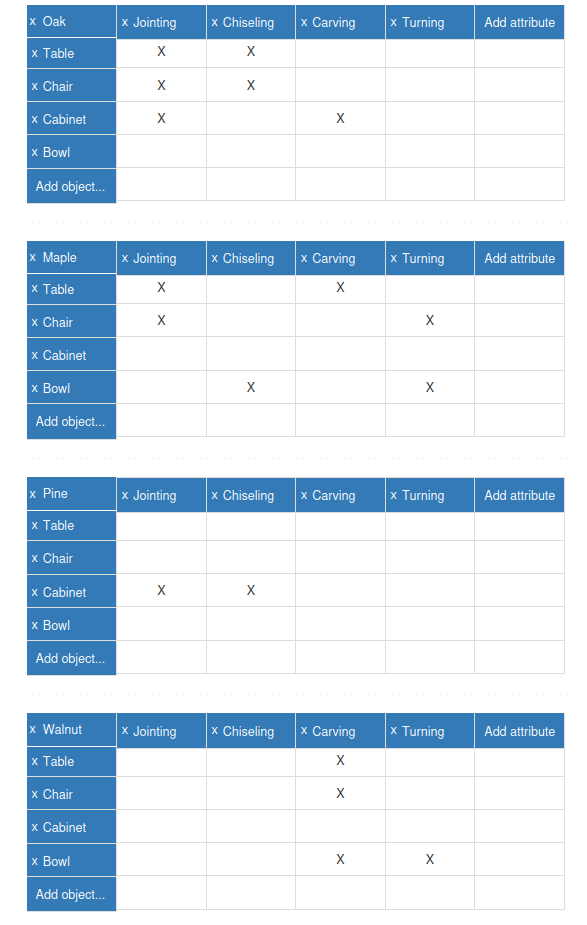
\includegraphics[width=0.5\textwidth]{context.png}
  \caption{Woodworking Triadic Context}
  \label{fig:context}
\end{figure}

\begin{figure}[htbp]
  \centering
  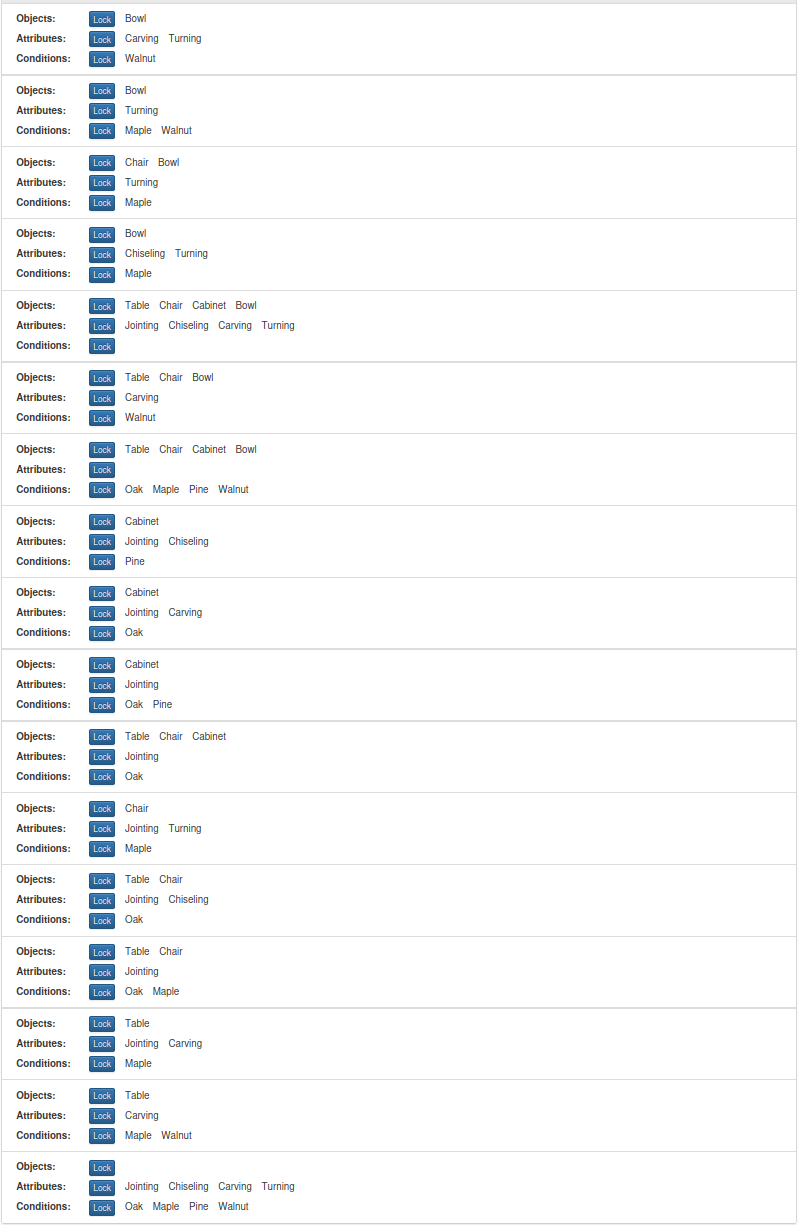
\includegraphics[width=0.9\textwidth]{concepts.png}
  \caption{Woodworking Triadic Concepts}
  \label{fig:context}
\end{figure}

\newpage
\textbf{Starting triconcept}: (Bowl, \{Carving, Turning\}, Walnut), along the condition dimension: Walnut

\begin{figure}[htbp]
  \centering
  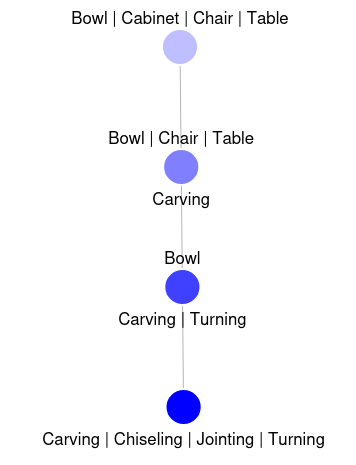
\includegraphics[width=0.5\textwidth]{cluster_0.png}
  \caption{Starting cluster, along condition dimension}
  \label{fig:cluster_0}
\end{figure}

\newpage
\textbf{Navigation Step 1:} Selecting the (Bowl, \{Carving, Turning\}) concept, locking the object dimension

\begin{figure}[htbp]
  \centering
  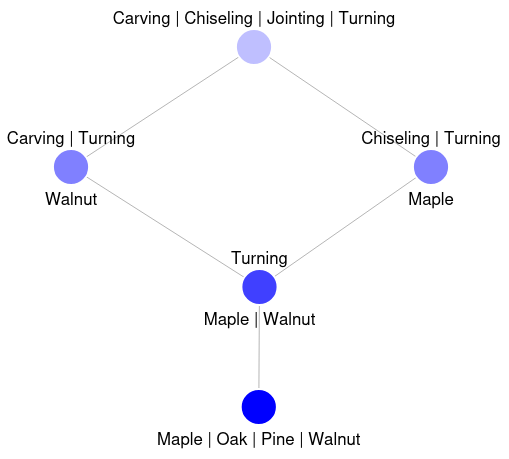
\includegraphics[width=0.5\textwidth]{cluster_1.png}
  \caption{Second cluster, from (Bowl, \{Carving, Turning\}) concept, along object dimension}
  \label{fig:cluster_1}
\end{figure}

\textbf{Navigation Step 2:} Selecting the (\{Carving, Turning\}, Walnut) concept, locking the attribute dimension, Carving

\begin{figure}[htbp]
  \centering
  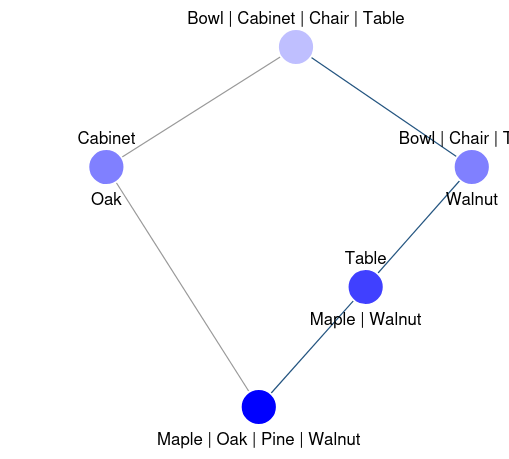
\includegraphics[width=0.5\textwidth]{cluster_2.png}
  \caption{Third cluster, from (\{Carving, Turning\}, Walnut) concept, along attribute dimension}
  \label{fig:cluster_2}
\end{figure}

\newpage
\textbf{Navigation Step 3:} Selecting the (Table, \{Maple, Walnut\}) concept, locking the condition dimension, Maple

\begin{figure}[htbp]
  \centering
  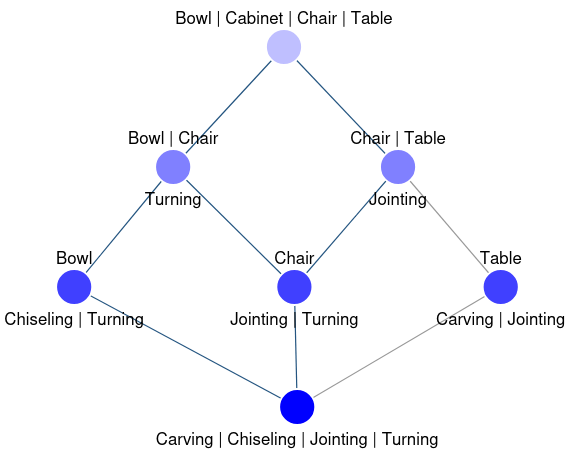
\includegraphics[width=0.5\textwidth]{cluster_3.png}
  \caption{Fourth cluster, from (Table, \{Maple, Walnut\}) concept, along condition dimension}
  \label{fig:cluster_3}
\end{figure}

\textbf{Navigation Step 4:} Selecting the (Chair, \{Jointing, Turning\}) concept, locking the object dimension, Chair

\begin{figure}[htbp]
  \centering
  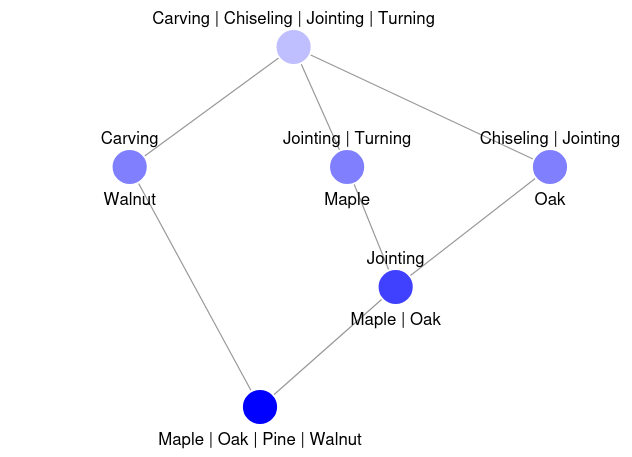
\includegraphics[width=0.5\textwidth]{cluster_4.png}
  \caption{Fifth cluster, from (Chair, \{Jointing, Turning\}) concept, along object dimension}
  \label{fig:cluster_4}
\end{figure}


\newpage
\textbf{Navigation Step 5:} Selecting the (Jointing, \{Maple, Oak\}) concept, locking the attribute dimension, Oak

\begin{figure}[htbp]
  \centering
  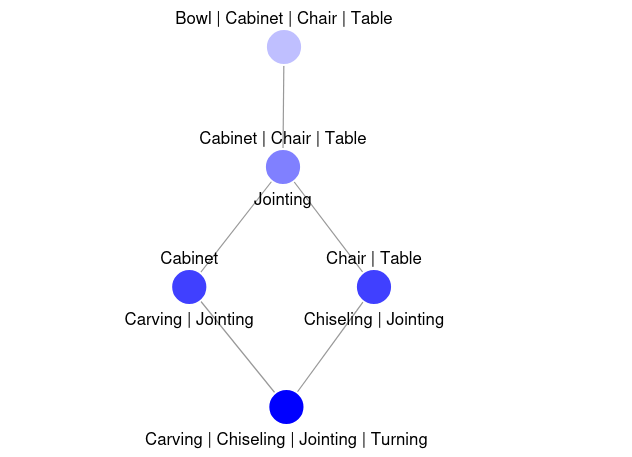
\includegraphics[width=0.5\textwidth]{cluster_5.png}
  \caption{Sixth cluster, from (Jointing, \{Maple, Oak\}) concept, along attribute dimension}
  \label{fig:cluster_5}
\end{figure}

This represents the second cluster from Fig \ref{fig:cluster_1}, let's try using the other attribute, Maple

\textbf{Navigation Step 5:} Selecting the (Jointing, \{Maple, Oak\}) concept, locking the attribute dimension, Maple

\begin{figure}[htbp]
  \centering
  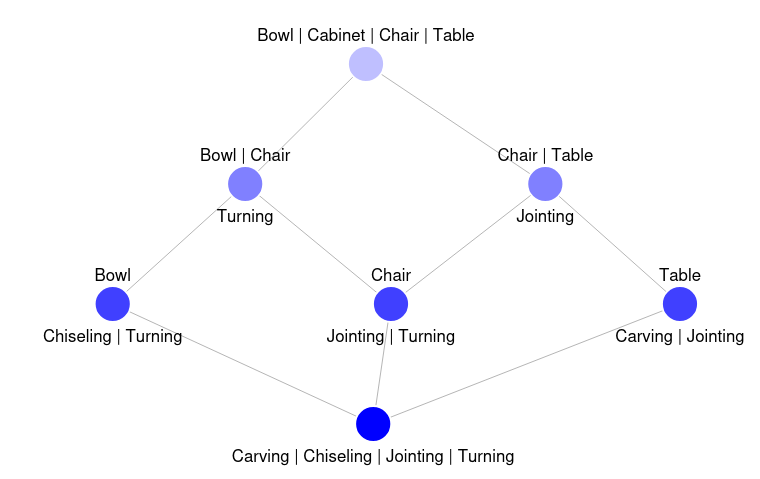
\includegraphics[width=0.5\textwidth]{cluster_5_2.png}
  \caption{Sixth cluster, from (Jointing, \{Maple, Oak\}) concept, along attribute dimension}
  \label{fig:cluster_5_2}
\end{figure}

This represents the fourth cluster from Fig \ref{fig:cluster_3}, let's try using the other attribute, Maple

\section*{Conclusion}
Found 5 clusters in approachabiliy graph, starting with (Bowl, \{Carving, Turning\}, Walnut) concept, along the Walnut condition dimension
\end{document}
